\documentclass{beamer}
%\documentclass[handout]{beamer} %% Ignoring pauses

\usepackage[utf8x]{inputenc}
\usepackage[english]{babel}
\usepackage{lstautogobble}
\usepackage{ragged2e}
\usepackage{listings}
\usepackage{pgfplots}
\usepackage{fdsymbol}
\usepackage{graphicx}
\usepackage{amsmath}

\usepackage{tikz}

\pgfplotsset{width=15cm,height=7cm,compat=1.7}
\usetikzlibrary{shapes.geometric, arrows}

\definecolor{nBlue}{RGB}{38,65,189}

\usetheme{default}
\usecolortheme{default}
\setbeamercolor{headFoot}{fg=white,bg=nBlue}

\setbeamerfont{footnote}{size=\tiny}

\setbeamertemplate{footline}{
  \leavevmode%
  \hbox{%
  \begin{beamercolorbox}[wd=.8\paperwidth,ht=2.25ex,dp=1ex,left]{headFoot}%
    \hspace*{2ex}\insertshorttitle
  \end{beamercolorbox}%
  \begin{beamercolorbox}[wd=.2\paperwidth,ht=2.25ex,dp=1ex,right]{headFoot}%
    \insertframenumber{}/\inserttotalframenumber\hspace*{2ex}
  \end{beamercolorbox}}%
  \vskip0pt%
}

\setbeamertemplate{frametitle}{\vskip-3pt
  \leavevmode
  \hbox{%
  \begin{beamercolorbox}[wd=\paperwidth,ht=5ex,dp=1ex]{headFoot}%
    \hspace*{1ex}\large\insertframetitle \\
    \hspace*{1.31ex}\scriptsize\insertframesubtitle
  \end{beamercolorbox}
  }%
}

\setbeamertemplate{navigation symbols}{}
\setbeamertemplate{caption}[numbered]
\setbeamercolor*{title}{use=structure,fg=white,bg=nBlue}
\setbeamertemplate{title page}[default][colsep=-4bp,rounded=false,shadow=false]

%%
\tikzstyle{rec}   = [rectangle, rounded corners, draw=nBlue, fill=nBlue!30,
text width=3cm, text centered, minimum height=1cm]
\tikzstyle{marks} = [text width=4cm, inner sep=0pt]
\tikzstyle{arrow} = [->, >=latex, draw=nBlue]

%% Agda and Haskell colors
\definecolor{DarkOrange3}{RGB}{205,102,0}
\definecolor{agdaPurple}{RGB}{160,32,240}
\definecolor{DarkGreen}{RGB}{0,100,0}
\definecolor{DarkRed}{RGB}{139,0,0}
\definecolor{MediumBlue}{RGB}{0,0,205}
\definecolor{DeepPink2}{RGB}{238,18,137}

\lstdefinelanguage{Agda}{
  keywords={data, where, record, constructor, field, open, infixl},
  keywordstyle=\color{DarkOrange3}\ttfamily,
  morekeywords={[2]{Set, skip, hanoi, rep, begin, cong, sym, succ, sym,
      moves, Monad, MonadCount, MonadNonDet, MonadExcept, work, fastProd,
      pureFastProd, product, if, then, else, List, elem}},
  keywordstyle={[2]{\color{MediumBlue}\ttfamily}},
  morekeywords={[3]{mkMonad, mkMonadCount, mkMonadExcept, tt, zero, suc, refl}},
  keywordstyle={[3]{\color{DarkGreen}\ttfamily}},
  morekeywords={[4]{return, unity, left, right, associativity, tick, catch,
      fail}},
  keywordstyle={[4]{\color{DeepPink2}\ttfamily}},
  % moredelim=[is][\color{gray}]{@}{@},
  basicstyle=\fontfamily{dejavu}\selectfont\ttfamily\tiny\color{black},
  literate={
    {->}     {{$\rightarrow$}}2
    {oC}     {{$\circ$}}2
    {Aa}     {{$\forall$}}2
    {lam}    {{$\lambda$}}1
    {_1}     {{{\color{MediumBlue}$_1$}}}1
    {-fail1} {{{\color{DeepPink2}$-$fail$_1$}}}5
    {-fail2} {{{\color{DeepPink2}$-$fail$_2$}}}5
    {-catch} {{{\color{DeepPink2}$-$catch}}}5
    {-return}{{{\color{DeepPink2}$-$return}}}6
    {-1}     {{{\color{MediumBlue}$-1$}}}2
    {-mn}    {{{\color{MediumBlue}$-$mn}}}3
    {>>}     {{{\color{MediumBlue}$\gg$}}}2
    {>>=}    {{{\color{DeepPink2}$\gg=$}}}3
    {\{\{}   {{{\color{MediumBlue}$\langle$}}}1
    {\}\}}   {{{\color{MediumBlue}$\rangle$}}}1
    {[}      {{{\color{DarkGreen}[}}}1
    {]}      {{{\color{DarkGreen}]}}}1
    {::}     {{{\color{DarkGreen}::}}}2
    {-N}     {{{\color{MediumBlue}$\dotminus$}}}1
    {+}      {{{\color{MediumBlue}$+$}}}1
    {*}      {{{\color{MediumBlue}*}}}1
    {Tt}     {{{\color{MediumBlue}$\top$}}}1
    {bN}     {{{\color{MediumBlue}$\mathbb{N}$}}}1
    {bZ}     {{{\color{MediumBlue}$\mathbb{Z}$}}}1
    {qed}    {{{\color{MediumBlue}$\blacksquare$}}}1
    {==}     {{{\color{MediumBlue}$\equiv$}}}2
    {0}      {{{\color{agdaPurple}0}}}1
    {1}      {{{\color{agdaPurple}1}}}1
    {2}      {{{\color{agdaPurple}2}}}1
    {3}      {{{\color{agdaPurple}3}}}1
    {4}      {{{\color{agdaPurple}4}}}1
    {5}      {{{\color{agdaPurple}5}}}1
    {6}      {{{\color{agdaPurple}6}}}1
    {7}      {{{\color{agdaPurple}7}}}1
    {8}      {{{\color{agdaPurple}8}}}1
    {9}      {{{\color{agdaPurple}9}}}1
  },
  identifierstyle=\ttfamily\color{black},
  sensitive=true,
  comment=[l]{--|},
  commentstyle=\color{DarkRed}\ttfamily,
  stringstyle=\color{MediumBlue}\ttfamily,
  autogobble=true
}

\lstdefinelanguage{Haskell}{
  keywords={module, where, import, class, if, then, else},
  keywordstyle=\color{agdaPurple}\ttfamily,
  morekeywords={[2]{:, =, -, >}},
  keywordstyle={[2]{\color{DarkRed}\ttfamily}},
  morekeywords={[3]{Monad}},
  keywordstyle={[3]{\color{DarkGreen}\ttfamily}},
  basicstyle=\tiny,
  literate={
    {->} {{{\color{DarkRed}$\rightarrow$}}}2
    {::} {{{\color{DarkRed}::}}}2
    {>>=}{{{\color{DarkRed}$\gg=$}}}3
    {oC} {{$\circ$}}2
    {lam}{{$\lambda$}}1},
  identifierstyle=\ttfamily\color{black},
  sensitive=true,
  comment=[l]{--|},
  commentstyle=\color{DarkRed}\ttfamily,
  stringstyle=\color{MediumBlue}\ttfamily,
  autogobble=true
}

\lstset{escapeinside={@}{@},
  basicstyle=\fontfamily{dejavu}\selectfont\ttfamily\small\color{black}}

\renewcommand{\arraystretch}{1.2}
\justifying

\title{(Perhaps Less Simple) Monadic Equational Reasoning}
\author{Elisabet Lobo-Vesga \\ Andr\'es Sicard-Ram\'irez}

\institute{Universidad EAFIT \\
Medellín, Colombia}
\date{January 2017}

\begin{document}

\begin{frame}
  \titlepage
\end{frame}

\begin{frame}{Introduction}
  \begin{figure}
    \centering
    \begin{tikzpicture}[thick, scale=0.7, transform shape]
      \node(Fp) [rec] {Pure functional programming};

      \visible<2->{\node(c) [marks, below of = Fp, yshift=-0.5cm]
        {\includegraphics[scale=0.06]{check.png} Equational reasoning};}

      \visible<3->{\node(w) [marks, below of = c]
        {\includegraphics[scale=0.06]{wrong.png} Computational effects};}

      \visible<4->{\node(m) [rec, below of = w, yshift=-1cm]
        {Monads\footnotemark $^{,}$ \footnotemark};}

      \visible<5->{\node(q) [inner sep=0pt, right of = w, xshift=3cm,
        yshift=-0.5cm]{\includegraphics[scale=0.15]{quest.png}};}

      \visible<6->{\node(Sm) [rec, right of = q, xshift=3cm]
        {Simple axiomatic\\approach\footnotemark};}

      \visible<7->{\node(v) [below of = Sm, yshift=-1.5cm]
        {\includegraphics[scale=0.15]{verification}};}

      \visible<7->{\node(v1) [below of = v]{Verification};}

      \visible<1->{
        \draw[dashed, rounded corners, black!30] (-2.5,1) rectangle (2.5,-3);}
      \visible<4->{\draw [arrow]        (w)  -- (m);}
      \visible<5->{\draw [draw=nBlue]   (m)  -| (q);}
      \visible<5->{\draw [arrow]        (q)  |- (c);}
      \visible<6->{\draw [arrow]        (q)  -- (Sm);}
      \visible<7->{\draw [arrow,dashed] (Sm) -- (v);}
    \end{tikzpicture}
    \only<4->{\footnotetext[1]{Moggi, E. (1991) Notions of computation and
        monads}}
    \only<4->{\footnotetext[2]{Wadler, P. (1995) Monads for functional
        programming}}
    \only<6->{\footnotetext[3]{Gibbons, J., \& Hinze, R. (2011) Just do it:
        simple monadic equational reasoning}}
  \end{figure}
\end{frame}

\begin{frame}[fragile]{Simple Monadic Equational Reasoning}
  \begin{figure}
    \centering
    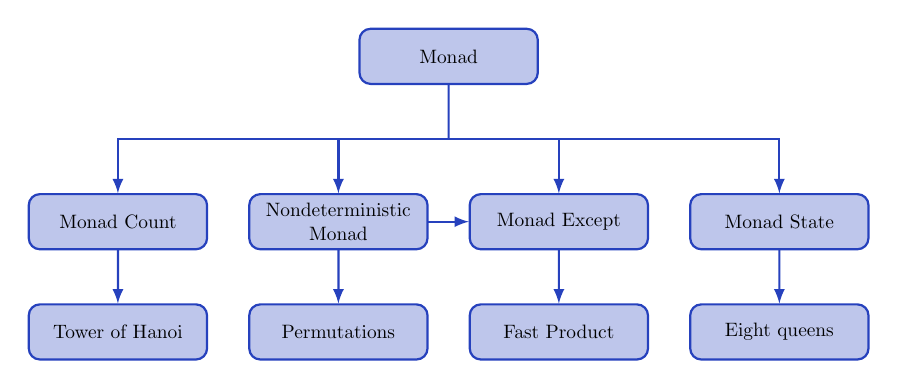
\begin{tikzpicture}[thick, scale=0.7, transform shape]
      \node(Mc)  [rec] {Monad Count};
      \node(Mnd) [rec, xshift=3cm, right of = Mc ]{Nondeterministic Monad};
      \node(Me)  [rec, xshift=3cm, right of = Mnd]{Monad Except};
      \node(Ms)  [rec, xshift=3cm, right of = Me ]{Monad State};

      \node(Mm)  [rec, xshift=2cm, yshift=2cm , above of = Mnd]{Monad};

      \node(Ha)  [rec, yshift=-1cm, below of = Mc] {Tower of Hanoi};
      \node(Perm)[rec, yshift=-1cm, below of = Mnd]{Permutations};
      \node(Fp)  [rec, yshift=-1cm, below of = Me] {Fast Product};
      \node(Eq)  [rec, yshift=-1cm, below of = Ms] {Eight queens};

      \draw [draw=nBlue] (Mm) -- (6,1.5);
      \draw [arrow] (6,1.5) -| (Mc);
      \draw [arrow] (6,1.5) -| (Mnd);
      \draw [arrow] (6,1.5) -| (Me);
      \draw [arrow] (6,1.5) -| (Ms);
      \draw [arrow] (Mc)    -- (Ha);
      \draw [arrow] (Mnd)   -- (Perm);
      \draw [arrow] (Mnd)   -- (Me);
      \draw [arrow] (Me)    -- (Fp);
      \draw [arrow] (Ms)    -- (Eq);
    \end{tikzpicture}
  \end{figure}
\end{frame}

\begin{frame}[fragile]{Monad}
  \begin{columns}[t]
    \begin{column}{.5\textwidth}
      \begin{block}{Haskell}
        \begin{lstlisting}[language=Haskell, mathescape]
          class Monad m where
            return :: a -> m a
            (>>=)  :: m a -> (a -> m b) -> m b
        \end{lstlisting}
      \end{block}
    \end{column}

    \begin{column}{.5\textwidth}
      \begin{block}{Properties}
        \begin{lstlisting}[language=Haskell, mathescape]
          return x >>= f   = f x
          mx >>= return    = mx
          (mx >>= f) >>= g =
              mx >>= (lam x -> f x >>= g)
        \end{lstlisting}
      \end{block}
    \end{column}
  \end{columns}

  \begin{block}{Agda}
    \begin{lstlisting}[language=Agda, mathescape]
      record Monad (M : Set -> Set) : Set_1 where
      constructor mkMonad

        field
          return : {A : Set} -> A -> M A
          _>>=_  : {A B : Set} -> M A -> (A -> M B) -> M B

          unity-left    : {A B : Set} {f : A -> M B} (x : A) ->
                          (return x) >>= f == f x

          unity-right   : {A : Set} (mx : M A) -> mx >>= return == mx

          associativity : {A B C : Set} {f : A -> M B} {g : B -> M C} (mx : M A) ->
                          (mx >>= f) >>= g == mx >>= (lam x -> f x >>= g)
    \end{lstlisting}
  \end{block}
\end{frame}

\begin{frame}[fragile]{Tower of Hanoi}
  \begin{figure}
    \includegraphics[scale=0.3]{hanoi}
  \end{figure}

  \begin{block}{Rules}
    \begin{enumerate}
    \item Only one disk can be move at a time
    \item A disk can only be moved if it's the uppermost disk on a stack
    \item No disk may be placed on top of a smaller disk
    \end{enumerate}
  \end{block}
\end{frame}

\begin{frame}[fragile]{Tower of Hanoi}
  \begin{columns}
    \begin{column}{.6\textwidth}
      \begin{block}{Recursive solution}
        \begin{itemize}
        \item Let $n$ be the total number of discs
        \item Number the discs from $1$ (topmost) to $n$ (bottom-most)
        \end{itemize}

        \begin{enumerate}
        \item Move $n-1$ discs from the source to the spare peg
        \item Move disk $n$ from the source to the target peg
        \item Move $n-1$ discs from the spare to the target peg
        \end{enumerate}
      \end{block}
    \end{column}

    \begin{column}{.4\textwidth}
      \begin{figure}
        \centering
        \includegraphics[scale=0.2]{recursive}
      \end{figure}
    \end{column}
  \end{columns}
\end{frame}

\begin{frame}[fragile]{Tower of Hanoi}
  \begin{block}{MonadCount}
    \begin{lstlisting}[language=Agda, mathescape]
      --| Supports effect of counting
      record MonadCount {M : Set -> Set} (monad : Monad M) : Set_1 where
        constructor mkMonadCount

          field
            tick : M Tt
    \end{lstlisting}
  \end{block}

  \begin{block}{Extra functions}
    \begin{lstlisting}[language=Agda, mathescape]
      --| Sequential composition
      _>>_ : {A B : Set} -> M A -> M B -> M B
      mx >> my = mx >>= lam _ -> my

      --| Identity computation
      skip : M Tt
      skip = return tt
    \end{lstlisting}
  \end{block}
\end{frame}

\begin{frame}[fragile]{Tower of Hanoi}
  \begin{block}{Implementation}
    \begin{lstlisting}[language=Agda, mathescape]
      --| Ticks the counter once for each move of a disc
      hanoi : bN -> M Tt
      hanoi zero    = skip
      hanoi (suc n) = hanoi n >> tick >> hanoi n

      --| Repeats a unit computation a fixed number of times
      rep : bN -> M Tt -> M Tt
      rep zero    mx = skip
      rep (suc n) mx = mx >> rep n mx
    \end{lstlisting}
  \end{block}

  \begin{block}{Properties of rep}
    \begin{lstlisting}[language=Agda, mathescape]
      rep-1  : (mx : M Tt) -> rep 1 mx == mx

      rep-mn : Aa m n -> (mx : M Tt) -> rep (m + n) mx == (rep m mx >> rep n mx)
    \end{lstlisting}
  \end{block}
\end{frame}

\begin{frame}[fragile]{Tower of Hanoi}
  \begin{block}{Proof}
    \begin{lstlisting}[language=Agda, mathescape]
      --| Solving a Tower of Hanoi of n disks requires (at least) @\textcolor{DarkRed}{2$^n$-1}@ moves
      moves : Aa n -> hanoi n == rep (2^n -N 1) tick
      moves zero    = refl
      moves (suc n) =
        begin
          (hanoi n >> tick >> hanoi n)
            =={{ cong f (moves n) }}
          (rep (2^n -N 1) tick >> tick >> rep (2^n -N 1) tick)
            =={{ cong g (sym (rep-1 tick)) }}
          (rep (2^n -N 1) tick >> rep 1 tick >> rep (2^n -N 1) tick)
            =={{ cong (lam x -> x >> r) (sym (rep-mn (2^n -N 1) 1 tick)) }}
          (rep (2^n -N 1 + 1) tick >> rep (2^n -N 1) tick)
            =={{ sym (rep-mn (2^n -N 1 + 1) (2^n -N 1) tick) }}
          rep ((2^n -N 1) + 1 + (2^n -N 1)) tick
            =={{ cong (lam x -> rep x tick) (sym (thm n)) }}
          rep (2^(n + 1) -N 1) tick
            =={{ cong (lam x -> rep (2^x -N 1) tick) (sym (succ n)) }}
          rep (2^(suc n) -N 1) tick
        qed
          where f = lam x -> x >> tick >> x
                r = rep (2^n -N 1) tick
                g = lam x -> r >> x >> r
    \end{lstlisting}
  \end{block}
\end{frame}

\begin{frame}[fragile]{Monad Except}
  \begin{lstlisting}[language=Agda, mathescape]
    record MonadExcept {M : Set -> Set} {Mnd : Monad M}
      (monad : MonadNonDet Mnd) : Set_1 where

      constructor mkMonadExcept

      field
        catch       : {A : Set} -> M A -> M A -> M A

        catch-fail1  : {A : Set} (h : M A) -> catch fail h == h

        catch-fail2  : {A : Set} (m : M A) -> catch m fail == m

        catch-catch  : {A : Set} (m h h' : M A) ->
          catch m (catch h h') == catch (catch m h) h'

        catch-return : {A : Set} (x : A) (h : M A) -> catch (return x) h == return x
  \end{lstlisting}
\end{frame}

\begin{frame}[fragile]{Monad Except}
  \begin{lstlisting}[language=Agda, mathescape]
    --| Computes the product of a list of Natural numbers
    productbN : List bN -> bN
    productbN []        = 1
    productbN (x :: xs) = x * productbN xs

    work : List bN -> M bN
    work xs = if (elem 0 xs) then fail else (return (productbN xs))

    fastProd : List bN -> M bN
    fastProd xs = catch (work xs) (return 0)

    pureFastProd : (xs : List bN) -> fastProd xs == return (productbN xs)

  \end{lstlisting}
\end{frame}

\begin{frame}{Conclusions}
\end{frame}
\end{document}